%% Projeto Apostila De Python para pessoas sem conhecimento prévio de porcaria nenhuma
%% mas que querem fazer bonito

%% O preâmbulo a seguir coloca o documento todo no formato ABNT puro.
%% Devido a interpretação local (das muitas possíveis) da ABNT, alguns
%% podem questionar o formato.

%% abtex2-modelo-livro.tex, v-1.9.7 
%% Copyright 2012-2018 by abnTeX2 group at http://www.abntex.net.br/
%%
%% This work may be distributed and/or modified under the
%% conditions of the LaTeX Project Public License, either version 1.3
%% of this license or (at your option) any later version.
%% The latest version of this license is in
%%   http://www.latex-project.org/lppl.txt
%% and version 1.3 or later is part of all distributions of LaTeX
%% version 2005/12/01 or later.
%%
%% This work has the LPPL maintenance status `maintained'.
%%
%% Further information is available on 
%% http://www.abntex.net.br/
%% 


\documentclass[
	% -- opções da classe memoir --
%	10pt,				% tamanho da fonte
	12pt,				% tamanho da fonte
	openright,			% capítulos começam em pág ímpar (insere página vazia caso preciso)
	twoside,			% para impressão em recto e verso. Oposto a oneside
	a4paper,			% tamanho do papel. 
	%a5paper,			% tamanho do papel. 
	% -- opções da classe abntex2 --
	%chapter=TITLE,		% títulos de capítulos convertidos em letras maiúsculas
	%section=TITLE,		% títulos de seções convertidos em letras maiúsculas
	%subsection=TITLE,	% títulos de subseções convertidos em letras maiúsculas
	%subsubsection=TITLE,% títulos de subsubseções convertidos em letras maiúsculas
	% -- opções do pacote babel --
	english,			% idioma adicional para hifenização
	french,				% idioma adicional para hifenização
	brazil,				% o último idioma é o principal do documento
	sumario=tradicional
]{abntex2}

% compilação de fontes


\usepackage{mathtools}
\usepackage{amsfonts}
\usepackage{mathrsfs} % para mathscr

\usepackage{ifxetex}
\ifxetex
  % % se for utilizar as fontes do sistema: **escolha sua fonte**
    % comandos de fontes
\usepackage{mathspec}
\setmathsfont(Digits,Latin,Greek){Minion Pro}
\setmathrm{Minion Pro}
\setmainfont[Numbers=OldStyle]{Minion Pro} %fonte principal (serifada)
\setsansfont[Scale=0.9]{Myriad Pro} %fonte sem serifas
\setmonofont[Scale=MatchLowercase]{Consolas} % fonte monoespaçada
  
  \usepackage{polyglossia} %always load polyblossia after fonts for digits in math mode
  \setmainlanguage{brazil}
  \setotherlanguages{french,english,spanish,german,italian}  
  
\else
  % % se for utilizar pdflatex
\usepackage[utf8]{inputenc}
\usepackage{newtxmath} 
\usepackage{Alegreya}
\usepackage{AlegreyaSans}
\usepackage[lf]{FiraMono}
\usepackage[italic]{mathastext}
\fi

%% Observação: o pacote polyglossia pode apresentar erro ao ser utilizado com ifxetex + babel. 
%% Se isso acontecer, atualize o pacote para a versão mais recente ou utilize somente uma das sequências (pdflatex ou xelatex), comentando ou apagando a outra.

\usepackage{microtype} 				% para melhorias de justificação
\usepackage[dvipsnames]{xcolor} 		% para cores
\usepackage{graphicx} 			% para imagens
\usepackage{booktabs,tabularx,rotating}	% para tabelas
\usepackage{mdframed} 				% para caixas de texto como na CIP do verso do título
\usepackage{multicol}				% tabelas com colunas mescladas
\usepackage{lettrine}				% letras capitulares
\usepackage{xspace} 				% para nao precisar de espaços com {} depois de comandos
									% como \LaTeX e abreviações criadas pelo usuário
\usepackage{lipsum} 				% para texto de preenchimento de exemplo
\usepackage{leading}				% espaçamento entrelinhas (leading)
\leading{13pt}

% ---
% Pacotes de citações
% ---
\usepackage[brazilian,hyperpageref]{backref}	 % Paginas com as citações na bibl
\usepackage[alf]{abntex2cite}	% Citações padrão ABNT

% ---
% Configurações do pacote backref
% Usado sem a opção hyperpageref de backref
\renewcommand{\backrefpagesname}{Citado na(s) página(s):~}
% Texto padrão antes do número das páginas
\renewcommand{\backref}{}
% Define os textos da citação
\renewcommand*{\backrefalt}[4]{
	\ifcase #1 %
		Nenhuma citação no texto.%
	\or
		Citado na página #2.%
	\else
		Citado #1 vezes nas páginas #2.%
	\fi}%
% ---

% ---
% Informações do documento
% ---
\titulo{Apostila de Python Para Iniciantes}
\autor{Engenheiros que dizem: ``Nih!''}
\data{2020, v-0.0.0}
\preambulo{Breve sinopse da Apostila}
\local{Curitiba}
\instituicao{UTFPR}

% alterando o aspecto da cor azul
\definecolor{blue}{RGB}{41,5,195}

% informações do PDF
\makeatletter
\hypersetup{
     	%pagebackref=true,
		pdftitle={\@title}, 
		pdfauthor={\@author},
    	pdfsubject={\imprimirpreambulo},
	    pdfcreator={LaTeX with abnTeX2},
		pdfkeywords={abnt}{latex}{abntex}{abntex2}{livro}, 
		colorlinks=true,       		% false: boxed links; true: colored links
    	linkcolor=blue,          	% color of internal links
    	citecolor=blue,        		% color of links to bibliography
    	filecolor=magenta,      		% color of file links
		urlcolor=blue,
		bookmarksdepth=4
}
\makeatother
% ---


% ---
% Estilo de capítulos
%
% \chapterstyle{pedersen} 
% \chapterstyle{lyhne} 
%\chapterstyle{madsen} 
\chapterstyle{veelo} 
%
% Veja outros estilos em:
% https://www.ctan.org/tex-archive/info/MemoirChapStyles
% ---

% para cabeçalhos sem estar em maiúsculas
%\nouppercaseheads 

% -----
% Declarações de cabecalhos 
% -----
% Cabecalho padrao
\makepagestyle{abntbookheadings}
\makeevenhead{abntbookheadings}{\ABNTEXfontereduzida\thepage}{}{\ABNTEXfontereduzida\textit\leftmark}
\makeoddhead{abntbookheadings}{\ABNTEXfontereduzida\textit\rightmark}{}{\ABNTEXfontereduzida\thepage}
\makeheadrule{abntbookheadings}{\textwidth}{\normalrulethickness}

% Cabecalho do inicio do capitulo
\makepagestyle{abntbookchapfirst}
\makeoddhead{abntbookchapfirst}{}{}{}

% Configura layout para elementos textuais
\renewcommand{\textual}{%
  \pagestyle{abntbookheadings}%
  \aliaspagestyle{chapter}{abntbookchapfirst}% customizing chapter pagestyle
  \nouppercaseheads%
  \bookmarksetup{startatroot}% 
}
% ---



% Margens do documento 
%% (margens do abntex2 não combinam nem com A5 nem com estilos de capítulo da
% classe memoir.)
\setlrmarginsandblock{2.5cm}{3.5cm}{*}
\setulmarginsandblock{2.5cm}{3.5cm}{*}
\checkandfixthelayout
% ---


%% para inserção de trechos de código Python
\usepackage{pythonhighlight}

% ---
% Início do documento
% ---
\begin{document}
\frenchspacing

\frontmatter

% ---
% Capa principal
% ---
\begin{titlingpage}
\phantom{xxx}
\vspace{0.5cm}
\huge
\raggedright
\imprimirautor\\
\vspace{2.5cm}
\huge 
{\raggedleft
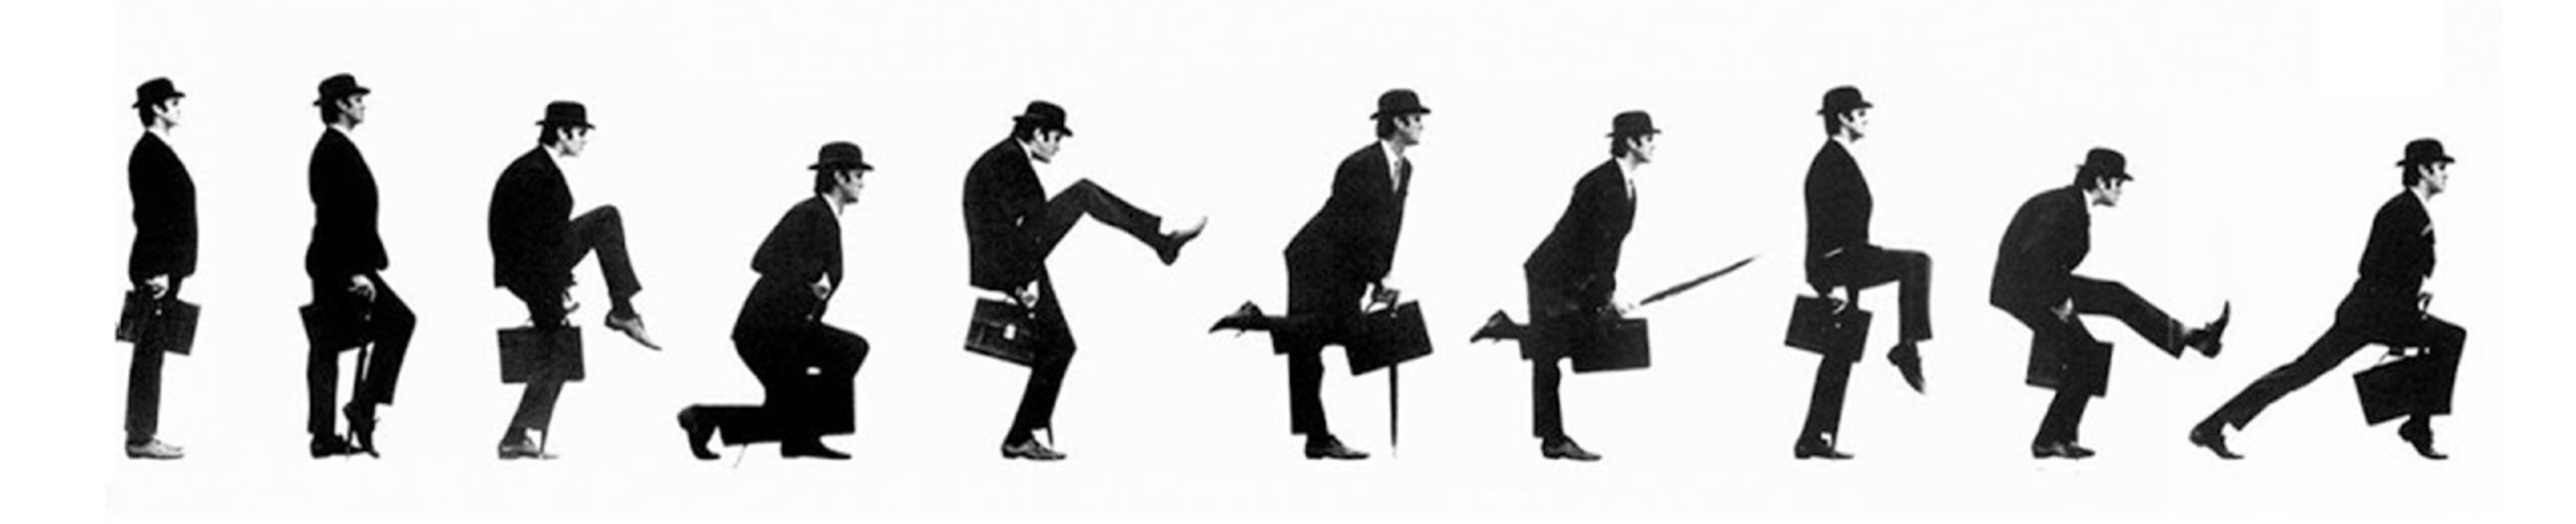
\includegraphics[scale=0.3]{MontyPythonSillyWalkDiagram.pdf}\\[1cm]
%%\includegraphics[scale=0.9]{abntex2-modelo-img-marca.pdf}\\[1cm]
\textit{\textcolor{blue}{\imprimirtitulo}}\\[1cm]
}
\centering 
% %este é um símbolo que só aparecerá com a fonte Minion.
\vfill
\Large
% %este é um símbolo que só aparecerá com a fonte Minion.
\imprimirinstituicao
\end{titlingpage}
% ---

% ---
% Contra-capa
% ---
\begin{titlingpage}

\phantom{xxx}
\vspace{0.5cm}
\huge
\raggedright
\imprimirautor\\
\vspace{2.5cm}
\huge 
{\raggedleft
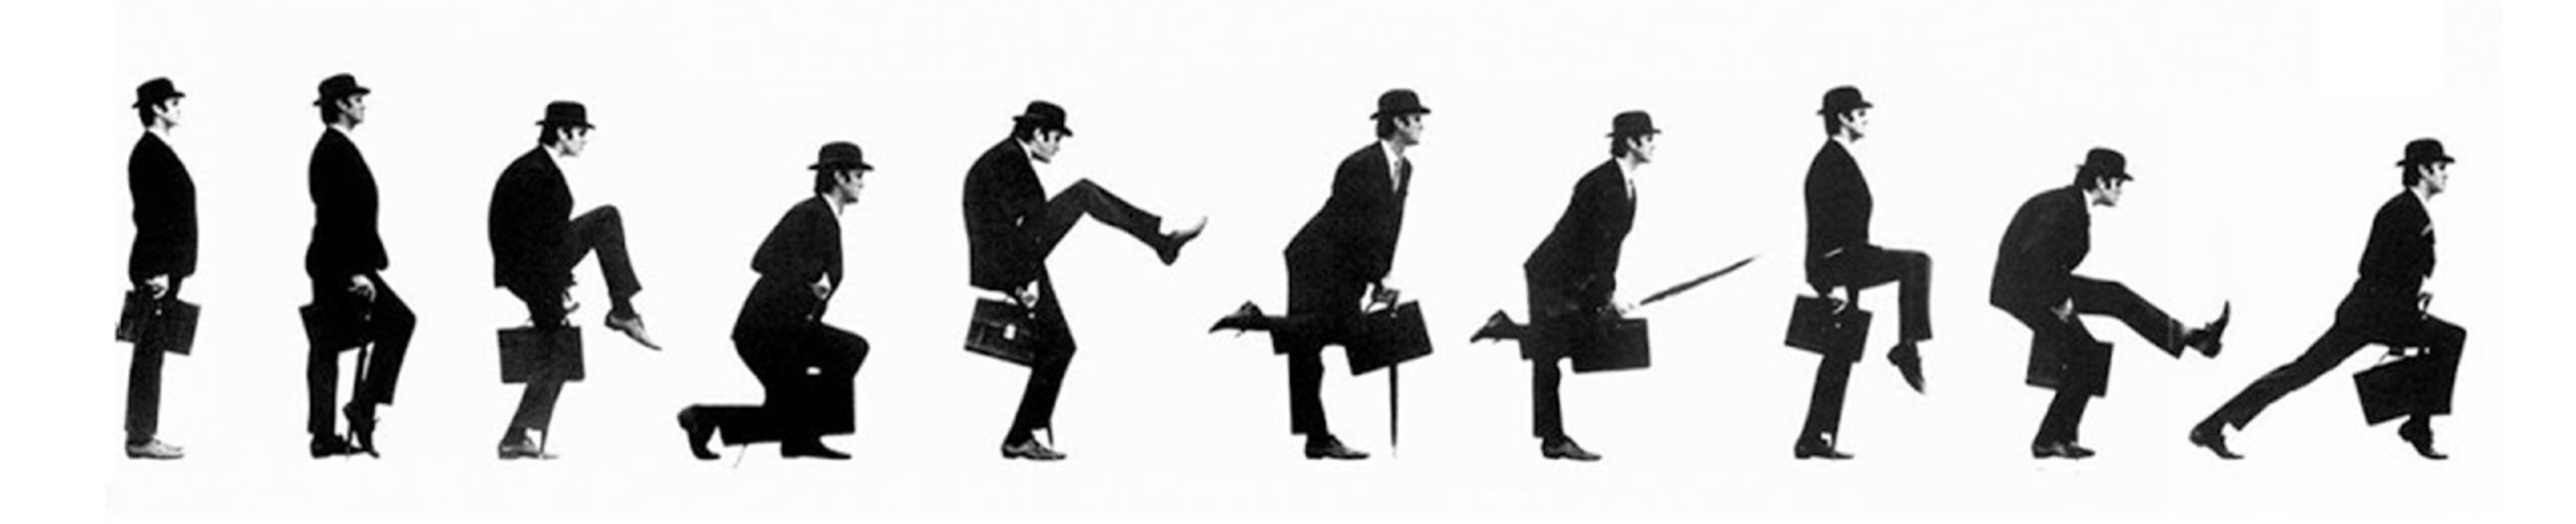
\includegraphics[scale=0.3]{MontyPythonSillyWalkDiagram.pdf}\\[1cm]
%%\includegraphics[scale=0.9]{abntex2-modelo-img-marca.pdf}\\[1cm]
\textit{\textcolor{blue}{\imprimirtitulo}}\\[1cm]
}
\centering 
% %este é um símbolo que só aparecerá com a fonte Minion.
\vfill
\Large
% %este é um símbolo que só aparecerá com a fonte Minion.
\imprimirinstituicao
% ---

% ---
% Verso da contra-capa
% ---
\clearpage
\ABNTEXfontereduzida
%\raggedright
© 2020 \imprimirautor \space \& \imprimirinstituicao
%este é só um exemplo de copyright.

Qualquer parte desta publicação pode ser reproduzida, desde que citada a fonte.

\vspace*{\fill}

\begin{center}
Dados Internacionais de Catalogação na Publicação (\textsc{cip})
Câmara Brasileira do Livro, \textsc{sp}, Brasil
\end{center}

\begin{mdframed}
\noindent Zanelatto, Giovani. %% autor como referenciado em citações;

\imprimirtitulo. / \imprimirautor. -- \imprimirlocal: \imprimirinstituicao\ 
 2020.

\medskip

Bibliografia.

ISBN XXXX-XXXX-XX.

\medskip

1. Programas de computador. 2. Python. 3. Fundamentos. 4. Receitas.

\end{mdframed}

\end{titlingpage}
% ---

% ---
% inserir lista de ilustrações
% ---
\pdfbookmark[0]{\listfigurename}{lof}
\listoffigures*
\cleardoublepage

% ---
% inserir lista de tabelas
% ---
\pdfbookmark[0]{\listtablename}{lot}
\listoftables*
\cleardoublepage
% ---

% ---
% inserir o sumario
% ---
\pdfbookmark[0]{\contentsname}{toc}
\tableofcontents*
\cleardoublepage
% ---

% ------------------------------------------------------------
% Início da parte textual
% ------------------------------------------------------------
%\textual
\mainmatter
% ------------------------------------------------------------
\OnehalfSpacing
% ------------------------------------------------------------
\chapter*[Introdução]{Introdução} %% título do capitulo
\addcontentsline{toc}{chapter}{Introdução}  %% comando para colocar o título do capítulo no table of contents
% ------------------------------------------------------------

\lettrine[nindent=0.35em,lhang=0.40,loversize=0.3]{P}{hyton} foi criado em torno de 1990 por
 Guido van Rossum.
O nome Python foi uma homenagem a um seriado de comédia da rede BBC intitulado
 ``Monty Python's Flying Circus'', do qual Guido é fã \cite{Lutz}. 
 Curiosamente muitos autores e desenvolvedores preferem ser associados a cobras e serpentes 
 do que a um grupo de humor e cada vez menos se observam referências ao programa de humor na literatura.

Desde sua estréia pública em 1991, Python tem crescido e se atualizado;
 passando de uma linguagem de sript para uma ferramenta bem estabelecida e 
 amplamente utilizada por todo o globo. 
 \emph{Elaborar mais isto aqui, encher linguiça com o que for informação bacana, 
 mesmo que inútil, mas sem ser chato ou se alongar demais...}

Esta apostila tem como objetivo iniciar os que ainda não programam em linguagem alguma,
e capacitá-los a compreender e executar uma série de receitas para resolução de problemas práticos.
Referências básicas e avançadas serão indicadas para o estudante que quiser se aprofundar mais
ou estiver curioso para saber o que há debaixo do capô.

\section[Mas o que é Python?] {Mas o que é Python?}%\addcontentsline{toc}{section}{Mas o que é Python?}
Python é uma liguagem de computador interpretada. 
Isto significa que o computador, para executar um programa escrito em Python,
precisa necessariamente ter um interpretador de Python instalado. 
Linguagens compiladas não necessitam disto, embora eventualmente contem com a presença de 
bibliotecas como as do sistema operacional.

O fato de Python ser interpretado não deve ser interpretado como sinal de fraqueza. Linguagens compiladas são, de fato, mais versáteis e podem ser otimizadas a níveis que o Python não compete. Entretanto o Python contém uma quantidade enorme de módulos, escritos em linguagens compiladas e otimizados, de tal forma que boa parte das operações para as quais um módulo é utilizado, o interpretador não penaliza a velocidade. 

Portanto, antes de começar a desbravar o mundo da pro\-gra\-ma\-ção de computadores,
necessitaremos preparar o terreno e instalar alguma distribuição de Python. 
Muitas estão disponíveis, algumas com mais ou menos capacidades.
Indicamos uma distribuição em particular pois é mais fácil seguir o tutorial enquanto
não precisamos ficar perdendo tempo com questões do tipo: ``onde está o terminal de saída?''. 


\section[Mas por que Python?] {Mas por que Python?}%\addcontentsline{toc}{section}{Mas por que Python?}
\begin{itemize}
\item Python é fácil de aprender.
\item Python é versátil.
\item Python é poderoso.
\end{itemize}
\emph{Elaborar mais a lista de vantagens...}




% ------------------------------------------------------------
\chapter{Programação}
% ------------------------------------------------------------

% ------------------------------------------------------------
\section{Filosofia de Programação}
% ------------------------------------------------------------

Apesar de toda sua complexidade, um computador é tão inteligente quanto o programa que roda nele.
A grosso modo podemos dizer que um computador não passa de um ``estúpido muito rápido''.
Um computador não é capaz, por si só, de descobrir o que o usuário quer que ele faça.
Ao ligarmos um computador um pequeno programa na placa-mãe do computador faz uma checagem dos 
componentes instalados e inicia a execução de um programa no dispositivo de ``boot'', que carrega o que 
normalmente é o sistema operacional, que passa a ter o controle do sistema todo. 

O sistema operacional, seja ele qual for, estabelece a interface entre o usuário e o computador e também de 
interface entre programas e periféricos.
%ocupando-se de organizar e distribuir mensagens entre os diversos componentes e programas.
% Também é função do sistema operacional cuidar de detalhes de como desenhar um pixel na tela ou como
% se comunicar com uma impressora ou rede. 
Programas que executam sobre o sistema operacional não precisam 
saber qual a taxa de atualização dos pente de memória A, B ou C. Cabe ao sistema operacional servir de interface
entre um programa que manda desenhar uma figura na tela e a efetiva associação de valores na memória de vídeo
que faz com que a imagem de fato apareça desenhada na tela.

\emph{Cabe aqui uma ilustração do programa com uma figura e uma tela com a figura impressa.} 

Para organizarmos nossa contabilidade mensal com um computador, não basta ligá-lo e colocar a pilha
de extratos e informações sobre o teclado ou monitor. Ligamos o computador, que se inicializa e carrega
um sistema operacional e então escolhemos e executamos um programa aonde colocamos os dados e com 
o qual fazemos operações matemáticas e armazenamos o resultado. Programas complexos como o Microsoft Word, 
Windows 10, Ubuntu, IOS e Android, podem ter centenas de milhares de linhas de código. Programas não precisam 
ser complexos para serem úteis. Muito se pode fazer com poucas linhas de código, organização e imaginação.  

Com Python, podemos criar programas que acessam planilhas Excel e executam operações nestes valores sem a necessidade
de invocar comandos Excel. Podemos também criar arquivos Excel para testar se uma planilha realmente está funcionando 
conforme programado. 

Quando falamos em programas de computador, falamos em um conjunto lógico de instruções que instruem 
os vários macaquinhos do processador a fazer o que queremos que eles façam. A linguagem de programação estabelece
a interface entre o que sabemos escrever e o que os macaquinhos do processador compreendem.

O sucesso e a eficiência de um programa dependem essencialmente da habilidade lógica de quem define as operações
necessárias e sua ordem sequencial. Bons programadores procuram fazer códigos eficientes, o que é aprendido na prática
com a prática frequente da programação. \cite{Norton}

% ------------------------------------------------------------
\section{Sequencia lógica de ações}
% ------------------------------------------------------------

If we took the bones out, it wouldn't be crunchy, would it? I told you to lay off the beans, you whore! At this time, a friend shall lose his friend's hammer and the young shall not know where lieth the things possessed by their fathers that their fathers put there only just the night before, about eight o'clock. Well, had I got as far as the penis entering the vagina? Pero las llamas son peligrosas. Si usted ve una llama donde hay gente nadando, usted gritar: ¡Cuidado! ¡Llamas! And Dinsdale says 'I hear you've been a naughty boy, Clement', and he splits me nostrils open, saws me leg off and pulls me liver out. And I tell him 'My name's not Clement', and then he loses his temper and nails my head to the floor. Well, I think I should point out first, Brian, in all fairness, we are not, in fact, the rescue committee. However, I have been asked to read the following prepare statement on behalf of the movement. "We the People's Front of Judea, brackets, officials, end brackets, do hereby convey our sincere fraternal and sisterly greetings to you, Brian, on this, the occasion of your martyrdom."

Oh, waiter! This conversation isn't very good. I'm not a roman mum, I'm a kike, a yid, a heebie, a hook-nose, I'm kosher mum, I'm a Red Sea pedestrian, and proud of it! Well, er, yes Mr. Anchovy, but you see your report here says that you are an extremely dull person. You see, our experts describe you as an appallingly dull fellow, unimaginative, timid, lacking in initiative, spineless, easily dominated, no sense of humour, tedious company and irrepressibly drab and awful. And whereas in most professions these would be considerable drawbacks, in chartered accountancy, they're a positive boon. Shut your festering gob, you tit! Your type really makes me puke you vacuous, toffy-nosed, malodorous pervert!

It's not pining, it's passed on! This parrot is no more! It has ceased to be! It's expired and gone to meet its maker! This is a late parrot! It's a stiff! Bereft of life, it rests in peace! If you hadn't nailed it to the perch, it would be pushing up the daisies! It's metabolic processes are now history! He's off the twig! He's kicked the bucket, he's shuffled off the mortal coil, rung down the curtain and joined the choir invisible. This is an ex-parrot!

 
%
%A filosofia básica de qualquer linguagem de programação é baseada nas características básicas
%de todo o programa.
%\begin{itemize}
%	\item Programas servem para resolver problemas (não para criar outros).
%	\item Programas devem ser eficientes.
%	% \item Programas devem 
%\end{itemize}


\section{Instalando o que é preciso para Python}



\chapter{Elementos básicos de Python}

\section{Primeiro programa}
%\usepackage{pythonhighlight} %% google ctan
\begin{python}
def f(x):
    return x
\end{python}




% ------------------------------------------------------------
\postextual % pós-textual
% ------------------------------------------------------------

% ------------------------------------------------------------
\bibliography{Apostila_Python_References}
\end{document} %% documento termina aqui

% ------------------------------------------------------------
\chapter{Exemplos de imagens}
% ------------------------------------------------------------

\lipsum[1]

\begin{figure}
\centering
\includegraphics[width=0.6\linewidth]{example-image-a}
\caption{Exemplo de imagem.}
\label{fig:exemplo}
\end{figure}

\lipsum[6]





\lipsum[7]

% ------------------------------------------------------------
\chapter{Exemplos de tabela}
% ------------------------------------------------------------

\section{Uma seção}

\lipsum[8]

\begin{table}
\caption{Pequeno vocabulário de design de livros\label{vocabulario-texto}}
\ABNTEXfontereduzida
\begin{tabular}{p{4cm}p{4cm}}
\toprule
\textit{Termo em inglês} & \textit{Termo em português}\\
\midrule
\ABNTEXfontereduzida
title page & folha de rosto.\\

cover & capa\\

back cover & quarta capa ou contra-capa ou verso da capa\\

bastard title ou half title & falsa folha de rosto. Tem só o título do livro.\\

table of contents & sumário\\

text block ou book block & miolo\\

print space (alemão: \textit{Satzspiegel}) & mancha gráfica\\

section, gathering, quire (especialmente se não impresso), signature & caderno\\

leaf = folio (latim) & folha, composta de recto (lat.) (anverso/frente) e verso (lat.) (verso). Geralmente o recto é página ímpar, e verso é página par.\\

hardcover & capa dura.\\

endpaper/endsheet & folha de guarda. Folha de papel para prender o miolo do livro na capa dura.\\

dust jacket, dust cover, book jacket, dust wrapper & sobrecapa. Geralmente de papel, para cobrir capas duras.\\

front matter & parte pré-textual.\\

main matter & parte textual\\

back matter & parte pós-textual. Composta por epílogo, posfácio, apêndice, glossário, bibliografia, índice remissivo (inglês: index), colofão etc.\\

colophon & colofão. Breve descrição sobre aspectos da publicação do livro. \\

running headers & títulos correntes\\

volume & volume. Conjunto de páginas encadernadas.\\

\bottomrule
\end{tabular}
\footnotesize Fontes:\\
\url{http://pt.wikipedia.org/wiki/Design_de_livros}\\
\url{http://en.wikipedia.org/wiki/Book_design}\\
\url{http://static.lexicool.com/dictionary/RX7KW614433.pdf}\\
\end{table}


\begin{table}
\caption{Exemplo de tabela utilizando o pacote \textsf{booktabs}.}
\centering
\begin{tabular}{llr}
\toprule
\multicolumn{2}{c}{Item} \\
\cmidrule(r){1-2}
Animal    & Description & Price (\$) \\
\midrule
Gnat      & per gram    & 13.65      \\
          & each        & 0.01       \\
Gnu       & stuffed     & 92.50      \\
Emu       & stuffed     & 33.33      \\
Armadillo & frozen      & 8.99       \\
\bottomrule
\multicolumn{3}{l}{\ABNTEXfontereduzida Fonte: \url{http://en.wikibooks.org/wiki/LaTeX/Tables}}
\end{tabular}
\end{table}

\lipsum[9]

% ------------------------------------------------------------
\postextual % pós-textual
% ------------------------------------------------------------

% ------------------------------------------------------------
\bibliography{Apostila_Python_References}
%\bibliography{abntex2-modelo-references} % insere o arquivo de bibliografia
% ------------------------------------------------------------

% ------------------------------------------------------------
% Colofão: última página com informações sobre a composição do livro.
\cleardoublepage
\thispagestyle{empty} 

Sinta-se convidado a participar do projeto \abnTeX! Acesse o site do projeto em
\url{http://www.abntex.net.br/}. Também fique livre para conhecer, estudar,
alterar e redistribuir o trabalho do ABN\TeX, desde que os arquivos modificados
tenham seus nomes alterados e que os créditos sejam dados aos autores originais,
nos termos da ``The \LaTeX\ Project Public
License''\footnote{\url{http://www.latex-project.org/lppl.txt}}.

Encorajamos que sejam realizadas customizações específicas deste documento.
Porém, recomendamos que ao invés de se alterar diretamente os arquivos do
\abnTeX, distribua-se arquivos com as respectivas customizações.
Isso permite que futuras versões do \abnTeX~não se tornem automaticamente
incompatíveis com as customizações promovidas. Consulte
\citeonline{abntex2-wiki-como-customizar} para mais informações.

\end{document}
